\title{Chum Populations}

\documentclass[12pt, one column]{article}
\usepackage{graphicx}
\usepackage{float}
\usepackage{enumitem}
\usepackage{lineno}
\linenumbers


\usepackage{natbib}

%\usepackage{fontspec}
%\setmainfont{Georgia}
%\setsansfont{Trebuchet MS}
%\setmonofont{Inconsolata}



\begin{document}
% \bibliographystyle{}

\section*{Outline}
\begin{itemize}

\item Genotyping duplicates
\begin{itemize}
\item Legacy of the salmonid WGD
\item uncharacterized regions of the genome 
\item first approach in salmon using next-gen seq data.
\end{itemize}

\item Genome scan
\begin{itemize}
\item Puget Sound chum salmon populations
\begin{itemize}
\item Population structure
\item chum salmon anadromous life history - 
\item ESA listing - summer chum ESU
\item Effective population size
\end{itemize}

\item map-assisted, paired population design
\item draw on synteny / orthology to interpret results
\end{itemize}

\item Linkage Map
\begin{itemize}
\item consensus map
\item synteny
\item annotation
\end{itemize}

\end{itemize}
\pagebreak


\section*{Abstract}
The common ancestor of salmonids underwent a whole genome duplication (WGD) approximately 100 million years ago. Understanding the genetic legacy of this event is critical to the conservation and management of these economically and socially important fish species. In contrast to most animals with strictly disomic inheritance, regions of the salmon genome undergo tetrasomic inheritance.  Loci in these regions are often excluded from genetic analyses owing to increased complexity during both genotype assignment and subsequent analyses. Here I develop methods to better characterize the tetrasomically-inherited regions of salmonid genomes.


\section*{Introduction}

\subsection*{Genotyping duplicates}
Legacy of the salmonid WGD - Uncharacterized regions of the genome - retained through unknown mechanisms.  

Recent studies have shown the benefits of polyploidy in other species \citep{Selmecki2015}.  Possible benefits are unknown but could include reduced inbreeding depression in small isolated populations typical of salmonids.

This is the first time that high-throughput sequencing data has been applied to score duplicated loci within salmonids.

\subsection*{Genome scan}
map-assisted genome scan with a paired population design. The linkage map will be used to interpret the population genomic data. They provide information on the genomic adjacency of loci and facilitate the  assessment of statistical independence between alleles.  This can address the persistent problem of pseudoreplication, such as during the estimation of effective population size (e.g., \citet{Larson2014} or for marker development for mixed stock analysis. Kernel smoothing and bootstrapping (e.g., \citet{Hohenlohe2010} will be used to identify genomic regions with elevated level of divergence.

draw on synteny / orthology 

\subsubsection*{Puget Sound chum salmon}

Chum salmon (Oncorhynchus keta) have the widest distribution of any Pacific salmonid, from Korea, around the Pacific Rim, to Oregon \citep{Salo1991}. Chum salmon are abundant and are utilized by tribal and non-tribal fishers and comprise the dominant commercial fishery in Washington State. Recently some chum salmon populations have undergone drastic declines.  National Oceanic and Atmospheric Administration (NOAA) Fisheries recognizes four evolutionarily significant units (ESUs) of chum salmon in the Pacific Northwest. Of the four, two are listed as ‘threatened’ under the Endangered Species Act: the Hood Canal summer-run ESU and the Columbia River ESU. The Hood Canal summer-run ESU is composed of 16 historic populations, 7 of which are extinct \citep{Good2005} and is the earliest-returning chum salmon stock in the Americas. Further work on Population structure?

Two evolutionary significant units (ESU) - Hood canal summer-run vs the rest. 'Genetically and ecologically distinct' threatened under the ESA. Notice which populations where supplemented by hatchery programs?
Chum salmon stray at similar rates to other pacific salmon \cite{Small2014} (could also cite Johnson et. al. 1997).  Note past measures of Effective population size.

Salmonids in the Pacific Northwest have a rich variety of life histories, with variation in run-timing, straying rates, age at maturity, freshwater residence, and many other dimensions \citep{Quinn2005}. This species and population-level diversity adds resilience to ecosystems and to species of conservation and economic concern \citep{Schindler2010}, especially in the face of climate change (reviewed in \citet{Schindler2015}).  Life history differs across populations within Puget Sound.  Generally, eggs are deposited in November - December. Embryos devlope and hatch after ~4 months and migrate to sea. 'survival and growth in juvenile chum salmon depend less on freshwater conditions than on favorable estuarine and marine conditions.'  Chum salmon return to freshwater to spawn at 3-5 years of age, and generally spawn within 100km of the ocean.

\subsection*{Objectives}

\section*{Methods}

\subsection*{Sequence analysis}
Genetic variation was quantified with a reference-based approach using the \texttt{Stacks} software pipeline \citep{Catchen2013}.  A chum salmon reference constructed from \citep{Waples2015}. Reads from each individual were demultiplexed and quality filtered with 'process-radtags' and then aligned to the reference with BWA-mem  (version 0.7.5a-r405) \citep{Li2013}.  Alignments containing indels or with a mapping quality < 20 were removed. Stacks components \texttt{pstacks}, \texttt{cstacks}, \texttt{sstacks}, and \texttt{populations} were used to identify and genotype genetic variants for each population individual.

The initial set of genotypes and individuals was assessed prior to further analysis.  Loci or individuals with more than 25\% missing data were removed.  Loci with a minor allele frequency below 5\% were removed. Hardy-Weinberg equilibrium was tested within each collection using the mid p-value statistic \citep{Graffelman2013}. Loci rejecting HWE in more than 5 collections were removed.  Finally, within each RAD locus, only the single SNP with the largest minor allele frequency was retained, to reduced pseudo-replication caused by physical linkage.  All filters were applied in PLINK (version v1.90b3q) \citep{Chang2014}. Note that for for the dominant coding used for the PCA analyses of population structure (see below), sequence haplotypes containing all SNPs within each locus were utilized. See supplemental file XXX for detailed description of the analysis pipeline.

Paralogous loci were identified by through their segregation patterns as in \citet{Waples2015}.  At each locus, the observed allelic segregation pattern were fit to models specified by parental genotypes.

\subsection*{Linkage map}
We constructed a consensus linkage map from three gynogenetic haploid families (sizes 175, 34, 31) with the  LEPmap \citep{Rastas2013}. This linkage map  builds on the map presented in \citet{Waples2015} with the addition of two additional families and the placement of centromeric regions. As the linkage map is constructed from gynogenetic haploid offspring, it only reflects recombination events that occur within the female lineage. As with many other species, there are sex-specific differences in recombination rates. (Not sure what else to say about female/male differences in linkage maps). The position of centromeres within each chromosome will be estimated by measuring recombination fractions along chromosomes (cite Limborg?).

\subsection*{Individual-based analyses} 
Scoring paralogs using the dominance coding suggested by \citet{Patterson2006} for microsatellites. 

Principal component analyses (PCAs) were conducted with EIGENSOFT (version 6.0.1) \citep{Patterson2006}

PCAs were compared with a Procrustes analysis. When supplied with two PCA projections, this method attempts to find an optimal superimposition of both of them, this is achieved by  translation, rotation, reflection and scaling.  After this transformation is complete, the remaining difference in shape is a measure of the Procrustes distance between the projections \citep{Peres2001}.

Formal tests for population structure \citep{Patterson2006}, based on the Tracey-Widom distribution \citep{Tracy1994}. Q values.

\subsection*{Population-based analyses \& genome scans}
Allele frequencies, Heterozygosity, and Fst (Weir 1984) were calculated for each locus in PLINK.

Fst across the genome.  Use LOESS (local regression) to reveal regions of elevated differentiation.  Benefits of this approach vs a bootstrapping methods (eg. Hohenlohe 2010).

Genome scans.  Bayescan all populations - 
LFMM models with run-timing data

Effective population size was estimated for each population using the LD method implemented in the LDNe software package \citep{Waples2010}.  The LD methods estimates the average correlation of alleles at pairs of loci (r2). The mean pairwise r2 value across independently-assorting loci provides an estimate of contemporary effective population size. Only loci placed on the linkage map were used for this calculation and the map was utilized to ensure that only pairs of loci not co-located on a chromosome contributed to mean r2.

\subsection*{Synteny - relation to genetic resources}
By design, RADseq generates sequence data exclusively near restriction enzyme cut sites; alignments of RAD contigs to genomic resources relate RAD data to much larger genomic sections.  These resources often have functional annotations, whole gene sequences, and reading frame information that is unavailable to RADseq projects, expanding my ability to interpret genetic differentiation in a biological context.

(pending)
Contigs assembled from paired-end sequence data \citet{Waples2015} will be aligned to genomic resources including the Atlantic salmon genome (Willie Davidson, personal communication), chum transcriptome \citep{Seeb2011}

Othologous loci in Chinook salmon linkage maps of Chinook salmon (McKinney et al. submitted).  More detail on the Oxford grid construction and alignment parameters.

\subsection*{Should I do?}
phylogenetic tree


\section*{Results}
\subsection*{Sequencing and genotyping}
table of sequencing results -  by collection location, including family and wild samples.
Genotyping rate

\subsection*{Individual-based}


\subsection*{Population-based}
population structure

Summarize population relationships, consistent with \citet{Small2014}?

Breakdown of population structure and lower PC axes.

Four individual-based PCA figures

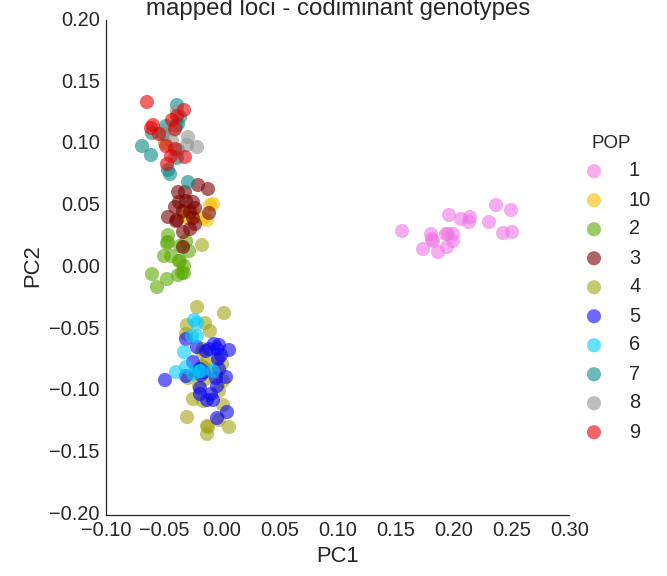
\includegraphics[scale=.3]{figures/PCA_codom.png}
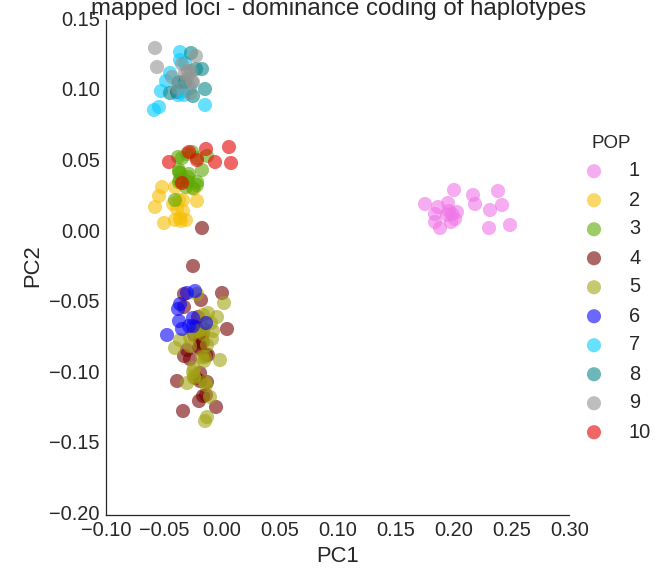
\includegraphics[scale=.3]{figures/PCA_dom.png}

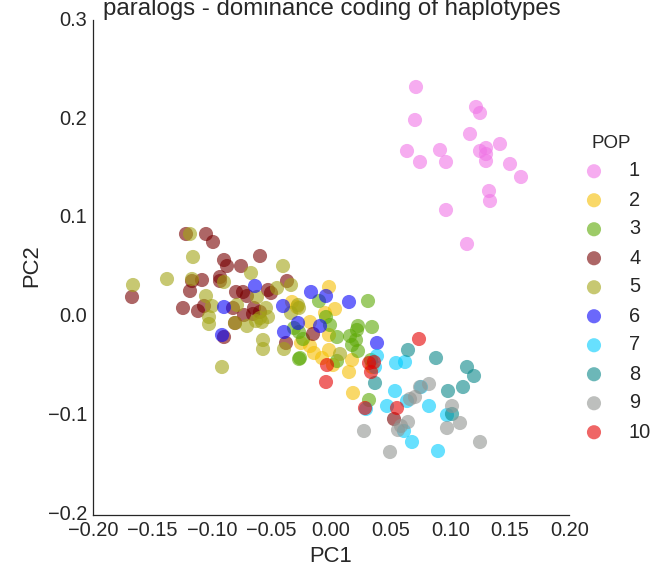
\includegraphics[scale=.3]{figures/PCA_dom_paralogs.png}
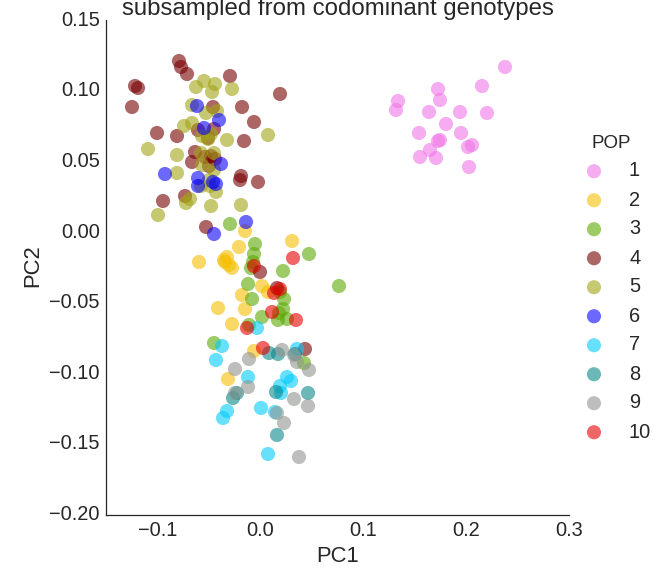
\includegraphics[scale=.3]{figures/PCA_codom_subsample.png}
Paralogs have similar neutral patterns of population structure (Procrustes similarity xxx)

Is the a possible quantitative measure of information loss due to dominance coding?  These doesn't quite make sense, as the the dominant haplotypes contain *more* information.

discuss population vs individual based results

can we demonstrate contained within paralogs by bootstrapping 
Genome scans - LG regions highlighted.

\subsection*{Effective population size}


Perhaps run the Ne with and without the linkage map correction?

\subsection*{Ascertainment Bias}
The linkage map was constructed from three female parents from Hoodsport hatchery, WA.

Demonstrate ascertainment effect when using only loci on linkage map - effect on allele frequencies.

\begin{figure}[H]
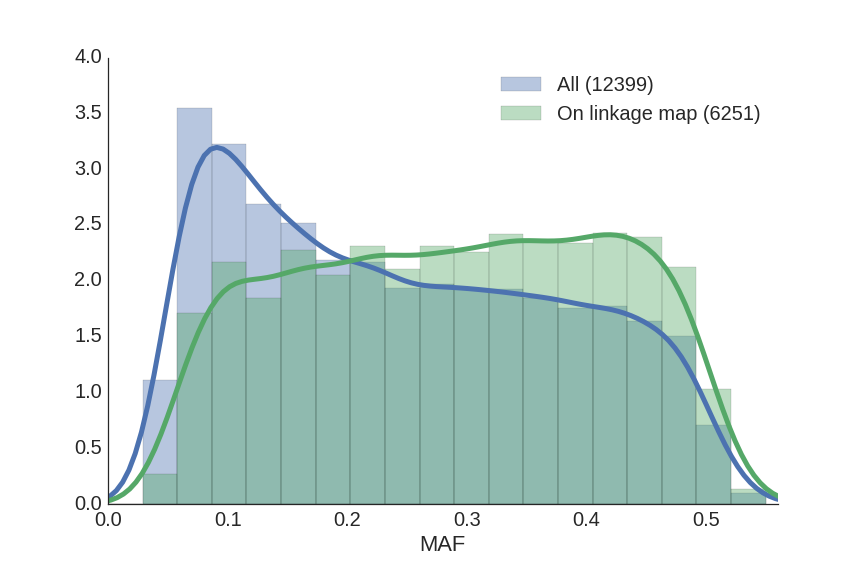
\includegraphics[scale=.3]{figures/supplemental/ascertainment2.png}
\caption{Minor allele frequency (MAF) density histograms for all loci (blue) and the subset of loci placed on the linkage map (green). The rightward shift in the MAF distribution shows the effect of ascertainment bias.} \textbf{TODO: align histogram bins, check the .5 boundary}
\end{figure}

\subsection*{Linkage map}
Here we present a consensus map placing 7795 loci onto 37 linkage groups.  These 37 linkage groups correspond 1:1 with those reported in \citep{Waples2015} and likely have a 1:1 correspondence with the 37 chromosomes in chum salmon \citep{Phillips2001}. \textbf{Do we want a map figure, perhaps just a slice of a single LG, or a table?}.

Of the 13,407 loci scored in the wild, 6,251 were placed on the linkage map. 

A total of xxx paralogs were identified and placed onto the linkage map (do I want to count them in pairs or not?).  The location of these paralogs were were concentrated on the distal ends of three chromosomes, consistent with results found in other Salmonid species  \citep{Brieuc2014, Kodama2014, Waples2015} (also McKinney submitted). Consistency across families (see supplemental table xx)

The consensus linkage map produced in chapter two will likely be similar to the single-family map produced in chapter one.  The map produced in chapter one contained thousands of loci placed on 37 linkage groups, with eight pairs of homeologous chromosome arms.  These pairs have elevated levels of sequence identity, likely due to ongoing tetrasomic inheritance.  We expect to find a similar pattern in the other two families, this would provide validation of the methods developed in chapter one. Potentially more interesting, but less likely, are drastic differences such as chromosomal inversions or chromosome number polymorphisms.  This type of chromosomal variation is documented within some salmon species \citep{Phillips2001}, but is not likely to be seen between these closely related families from Hoodsport Washington.

placement of centromeres

paralogs

Notice the distribution of paralogs matches the  pattern found in other salmonids.
syntenic/orthologous relationships, see supplemental figure xx.

Table (supplemental?)

\section*{Discussion}
To do

Compared to \citet{Small2014} the effective sizes (N$_{e}$) are larger, this could be due to the downward bias removed by utilizing the linkage map.

\section*{Meta}
Does this turn into two papers?

 - linkage map and individual-based analyses - including duplicated loci

 - inference of adaptation -associated  life history variation  - Fst across the genome.

\pagebreak
\section*{Supplemental Figures}

\begin{figure}[H]
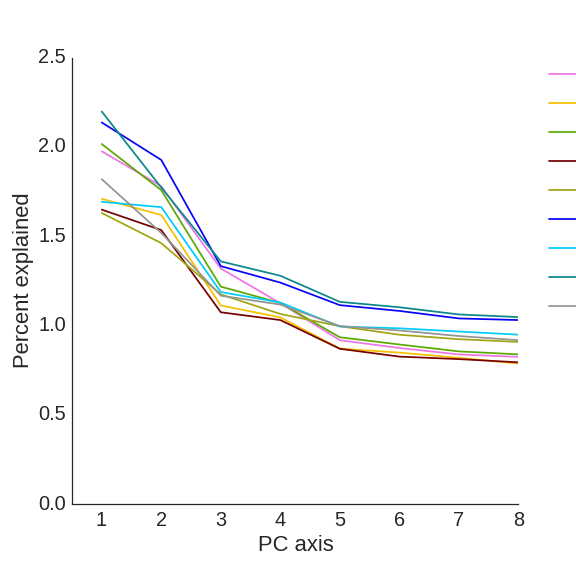
\includegraphics[scale=.4]{figures/supplemental/PCA_eigenvalues.png}
\caption{Percent variance explained (eigenvalue) for the first eight PC axes of each locus set.  Notice the similarity between the two bi-allelic sets and the two haplotypic sets.}
\end{figure}

\begin{figure}[H]
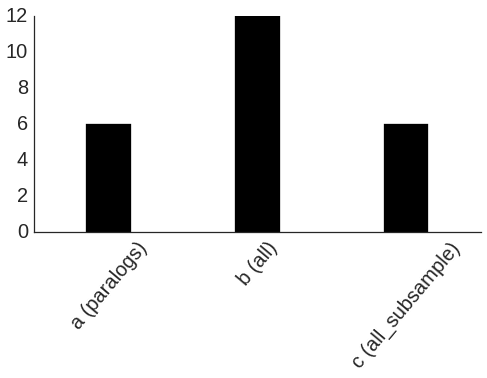
\includegraphics[scale=.4]{figures/supplemental/TW_stats.png}
\caption{Number of significant PC axes as determined by the Tracey-Widom test.}
\end{figure}

\begin{figure}[H]
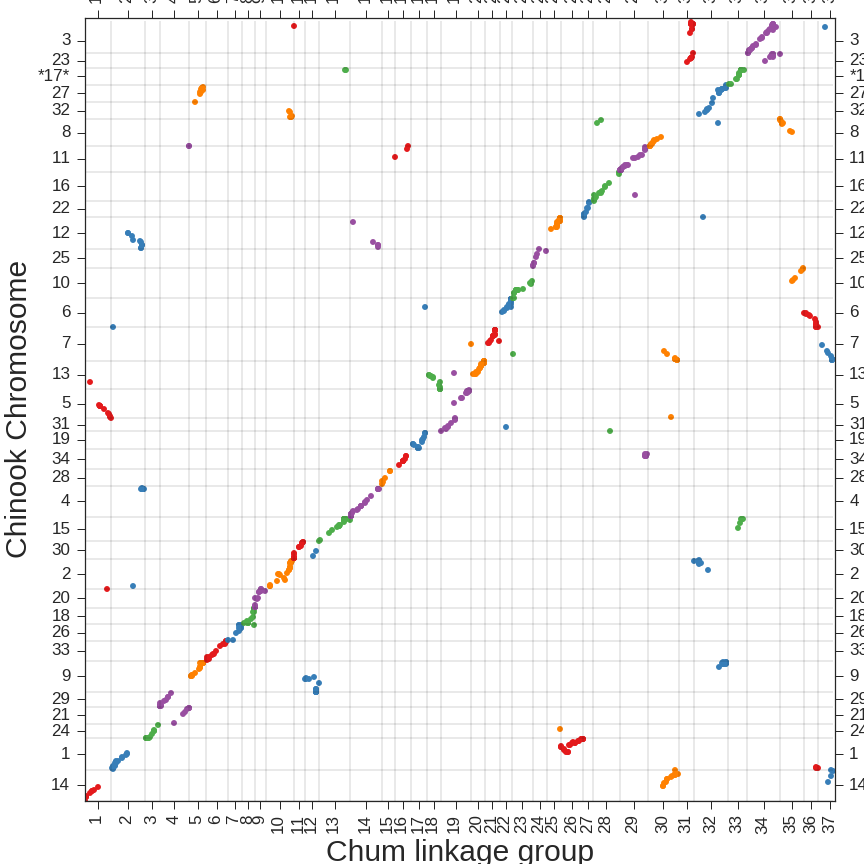
\includegraphics[scale=.25]{figures/supplemental/synteny_chinook.png}
\caption{Oxford grid - Chum and Chinook linkage groups. Loci are colored by their LG assignment in chum salmon and positioned according to the order within each genome.}
\end{figure}

% \section*{References}

\bibliographystyle{apalike}
\bibliography{./bibtex/7_13_15}

\section*{Acknowledgements}
Carita Pascal - lab work and library prep.

Seeb lab

WDFW - chum salmon expertise.

Rachel Hovel - multivariate stat advice.
\end{document}